\documentclass[final,3p,times]{elsarticle}
\usepackage{amsmath, amssymb, amsfonts, amsfonts, amsthm,latexsym}
\DeclareSymbolFont{yhlargesymbols}{OMX}{yhex}{m}{n}
\DeclareMathAccent{\overarc}{\mathord}{yhlargesymbols}{"F3}
\usepackage[mathscr]{euscript}
\usepackage[noend]{algorithmic}
\usepackage{comment}
\usepackage{algorithm}
\renewcommand{\algorithmiccomment}[1]{\hfill$\rhd$\textit{#1}}
\usepackage{graphics}
\usepackage{enumerate}
\usepackage{enumitem}
\usepackage[usenames]{color}
\usepackage{mathtools}
\usepackage[normalem]{ulem}
\usepackage{import}
\usepackage{comment}
\usepackage{wrapfig}
\usepackage{optidef}
\usepackage{epsfig}
\usepackage{tikz-cd}
\usepackage{color}
\DeclareMathOperator{\Tr}{Tr}
% Plots
\usepackage{graphicx}
\usepackage{float}
\usepackage[font=scriptsize,labelfont=bf]{caption}
\usepackage{subcaption}
\usepackage{url}
\usepackage{tikz}
\usetikzlibrary{positioning,chains,fit,shapes,calc}
\usepackage[all]{xy}

\newtheorem{theorem}{Theorem}[section]
\newtheorem{proposition}[theorem]{Proposition}%[section]
\newtheorem{lemma}[theorem]{Lemma}%[section]
\newtheorem{question}{Question}
\newtheorem{definition}{Definition}[section]
\newtheorem{fact}{Observation}[section]
\newtheorem{example}{Example}[section]
\newtheorem{corollary}[theorem]{Corollary}%[section]
\newtheorem{corollary*}{Corollary}%[section]
\newtheorem{remark}[theorem]{Remark}%[section]
\newtheorem{problem}{Problem}[section]
\newtheorem{observ}{Observation}

\newcommand{\TODO}[1]{\begingroup\color{red}#1\endgroup}
\def\TODOO#1{\marginpar{\tiny\raggedright\color{red}#1}}

\newcommand{\ak}[1]{\begingroup\color{orange}#1\endgroup}
\newcommand{\OLD}[1]{\begingroup\tiny\color{gray}#1\endgroup}
\newcommand{\PFS}[1]{\begingroup\color{blue}#1\endgroup}
\newcommand{\mh}[1]{\begingroup\color{magenta}#1\endgroup}

%\journal{Discrete Applied Mathematics}
%\journal{Journal of Combinatorial Theory, Series B}

\DeclareMathOperator{\lca}{lca}

\begin{document}

\begin{frontmatter}
  \title{How merging colors characterizes 3-BMGs}

  \author[LEI]{Annachiara Korchmaros}
  \ead{annachiara@bioinf.uni-leipzig.de}

  \author[STOCK]{Marc Hellmuth}
  \ead{marc.hellmuth@math.su.se}

  \author[LEI,LEI-other,MIS,TBI,BOG,SFI]{Peter F. Stadler}
  \ead{stadler@bioinf.uni-leipzig.de}

\address[LEI]{Bioinformatics Group, Department of Computer Science \&
  Interdisciplinary Center for Bioinformatics, Universit{\"a}t Leipzig,
  H{\"a}rtelstra{\ss}e 16-18, D-04107 Leipzig, Germany}

\address[STOCK]{Department of Mathematics, Faculty of Science,
Stockholm University, SE-10691 Stockholm, Sweden}

\address[LEI-other]{German Centre for Integrative Biodiversity Research
  (iDiv) Halle-Jena-Leipzig, Competence Center for Scalable Data Services
  and Solutions Dresden-Leipzig, Leipzig Research Center for Civilization
  Diseases, and Centre for Biotechnology and Biomedicine at Leipzig
  University at Universit{\"a}t Leipzig}

\address[MIS]{Max Planck Institute for Mathematics in the Sciences,
  Inselstra{\ss}e 22, D-04103 Leipzig, Germany}

\address[TBI]{Institute for Theoretical Chemistry, University of Vienna,
  W{\"a}hringerstrasse 17, A-1090 Wien, Austria}

\address[BOG]{Facultad de Ciencias, Universidad National de Colombia, Sede
  Bogot{\'a}, Colombia}

\address[SFI]{Santa Fe Institute, 1399 Hyde Park Rd., Santa Fe NM 87501,
  USA}


\begin{abstract}
  
\end{abstract}


\begin{keyword}
 Colored directed graphs; rooted trees; phylogenetic
  combinatorics; best matches
\end{keyword}

\end{frontmatter}

\sloppy

\section{Introduction}
In the last few years, a new method was developed for studying phylogenetic trees on $n$ species which encodes their properties into an $n$ vertex-colored directed graph, called best match graph (n-BMG).

The simplest case, $n=2$, was worked out thoroughly by exploiting the characterization of 2-BMGs by purely graph theoretic axioms; see \cite{Geiss:19a,Geiss:20b,Korchmaros:21a,korchmaros2021quasi,Schaller:21a,Schaller:21b,Schaller:21c,Schaller:21d}. For $n=3$, a graph theoretical characterization was also given under the rather restrictive hypothesis that all edges are symmetric~\cite{geiss2020reciprocal}. The general case, $n\ge 3$, appears to be more involved since neither analog characterization of an n-BMG in terms of graph theoretic axioms seems plausible, nor its induced 2-BMGs are enough to characterize it. Indeed, an n-colored digraph may not be a best match graph even if each of its $n(n-1)/2$ maximal inherited 2-colored subgraphs is a 2-BMG, as shown for $n=3$ in~\cite[Figure 1]{schaller2021corrigendum}. On the other hand, all 2-colored induced subgraphs of any BMG are necessarily 2-BMGs~\cite[Corollary 5]{Geiss:19a}, and this poses the question whether a BMG can be characterized by some family of its non-induced subgraphs which are 2-BMGs. Such non-induced subgraphs exist in any n-colored digraph $\Gamma$. In fact, preserving one color and merging the other $n-1$ colors into a new one gives an immediate example of a non-induced 2-colored subgraph with the same vertex set of $\Gamma$. We refer to this example as a \emph{color derivative} (subgraph) of $\Gamma$.

In this paper we investigate the above question for $n=3$. Our main contribution is the introduction of \emph{the 3-BMG condition} which ensures a 3-colored digraph to be a 3-BMG in terms of its color derivatives. This condition is not necessary in general, and our second contribution is describing a large family of 3-BMGs for which the 3-BMG condition is also necessary. To this aim, we forbid certain 3-colored digraphs on three vertices (F$^R$-graphs and F$^B$-graphs). 

The paper is organized as follows. In Section~\ref{sec:background}, we fix our notation and recall the definition and known characterizations of BMGs. The definition of a color derivative of a vertex-colored digraph is formalized in Section~\ref{sec:operators}, and the \emph{color-delta operator} $\Delta_{rb}$ is introduced which plays a role in Section~\ref{sec:3-BMG condition} to state the sufficiency of the 3-BMG condition; see Theorem~\ref{thm:sufficient_condition}. The study of the necessity part of the 3-BMG condition is carried out in Section~\ref{sec:nec_condition}. In particular, the concept of F$^R$-graph is introduced in Section~\ref{sec:forbidden_graphs} to find a large family of 3-BMGs characterized by the 3-BMG condition. Furthermore, a novel graph theoretical characterization for this family is presented in Theorem~\ref{thm:characterization3BMG_forbidden}. Forbidding F$^R$-subgraphs may be rephrased in terms of symmetric edges. Therefore, in Section~\ref{sec:sym_edges}, we provide some general results on the number of symmetric edges in a BMG.

\section{Background}
\label{sec:background}
\subsection{Vertex-colored digraphs}

\mh{
We consider \emph{directed graphs} $\Gamma=(V,E)$ with vertex set $V(\Gamma)\coloneqq V$ and edge set $E(\Gamma)\coloneqq E$
where $E\subseteq (V\times V)\setminus \{(x,x)\mid x\in V\}$. Hence, by definition, $\Gamma$ does not contain 
loops or multiple edges. We denote edges $e=(x,y)\in E$ simply by $xy$. For $xy\in E$, vertex $x$ is the \emph{tail} of $e$
and $y$ the \emph{head} of $e$. We call an edge $xy$ \emph{symmetric} if $yx\in E$. }
\OLD{
digraphs (directed graphs) are without loops and multiple edges. For a digraph $\Gamma$ with vertex set $\Gamma(V)$ and edge set $\Gamma(E)$, the notation $\Gamma=\Gamma(V,E)$ is also used. For $x,y\in V$,
the edge with tail $x$ and head $y$ is denoted by $xy$. If $xy,yx\in E$ then $xy$ (and $yx)$ is a {\emph{symmetric edge}}.
}

For a vertex $x\in V$, the out-neighbors and the in-neighbors of $x$ in $\Gamma$
are those vertices $z\in V$ for which $xz\in E$ and $zx\in E$, respectively. The
out-neighborhood of $x$ is denoted by $N_\Gamma(x)$, or 
\mh{simply by  $N(x)$ if there is no risk of confusion.}
\OLD{briefly by $N(x)$ when
this clearly refers to $\Gamma$.} A digraph $\Gamma$ is called sink-free if each
of its vertices has at least one out-neighbor.

\mh{
A \emph{directed path} from $x_0$ to $x_m$ in $\Gamma = (V,E)$ is a sequence of 
pairwise distinct vertices $x_0\rightarrow x_1 \rightarrow \cdots\rightarrow x_m
\rightarrow x_{m+1}$ such that $x_ix_{i+1}\in E$ for every
$0\le i \le m$. 
We call a sequence $x_0\rightarrow x_1 \rightarrow \cdots\rightarrow x_m\rightarrow  x_0$, $m\geq 2$
of vertices a directed cycle if  $x_0\rightarrow x_1 \rightarrow \cdots\rightarrow x_m$
is a directed path and $x_mx_0\in E$
The \emph{length} of a directed path or cycle is the number of its edges.
}

\TODO{MH: is $x\rightarrow y \rightarrow x$ to be considered as cycle? if so put 
$m\geq 1$ above instead of $m\geq 2$}

\OLD{\TODO{MH: cant see that this is ever used, so for now I made it shorter:}
A \emph{directed walk} from $x$ to $y$ in $\Gamma$ is a sequence of \mh{(not necessarily
distinct)} vertices
\OLD{$x=$} $x_0\rightarrow x_1 \rightarrow x_2 \rightarrow \cdots\rightarrow x_m
\rightarrow x_{m+1}$\OLD{$=y $} such that $x_ix_{i+1}\in E(\Gamma)$ for every
$0\le i \le m$. The \emph{length} of a directed walk is the number of its edges.
A directed walk in which all edges are distinct is called \emph{directed trail};
in particular, it is a \emph{directed path} when also all vertices are distinct.
A directed trail in which all vertices but the first and last are distinct is a
\emph{directed cycle}. 
}

Let $S$ be a finite set \mh{of colors}. \OLD{of size $n$ whose elements are called colors.} \OLD{If a}
\mh{A} digraph $\Gamma=(V,E)$ is colored by the colors in $S$, \OLD{then the} 
\mh{if there is a} surjective \mh{map}\OLD{color
function} $\sigma: V\to S$ \mh{where 
$\sigma(x)$ is called the \emph{color} of $x$. We use $(\Gamma,\sigma)$ to specify
that $\Gamma$ is equipped with such a map $\sigma$. A colored digraph $(\Gamma, \sigma)$ 
is \emph{properly colored} or, equivelently, $\sigma$ is a \emph{proper coloring}
of $\Gamma$, if $\sigma(x)\neq \sigma(y)$ for all $xy\in E$. }
If the neighborhood of any vertex contains
vertices for all colors, $\Gamma$ is \emph{color-sink free}. 


In this paper, we mostly concern with 3-colored digraphs, and we assume that the vertex colors to be red, blue and yellow. Therefore, the vertex set is partitioned in three \emph{color classes} as $V=R\,\dot{\cup}\, B\,\dot{\cup}\, Y$; we name such classes $R,B$ and $Y$ when they contain red, blue and yellow vertices, respectively. For a red vertex $x$, its out-neighbourhood $N(x)$ splits into two colored out-neighbourhoods, namely of blue and yellow vertices, denoted by $N^{B}(x)$ and $N^{Y}(x)$. 

\subsection{Rooted trees and triples}
Any acyclic undirected \TODO{undirected not clear, since mentioned above "only directed considered"} and connected graph is a tree. A tree $T$ is
\emph{rooted} whenever one of its vertices is named as root; in this case, we
use the symbol $\rho_T$, or briefly $\rho$, to indicate such a vertex.  

In this paper, $L=L(T)$ is the leaf set of a tree $T$. The notation $(T,\sigma)$ is customary when the leaves of $T$ are colored by the color map $\sigma$. There is a partial ordering $\preceq_T$ on $L(T)$ such that $x\preceq_T y$ holds if $y$ lies on the path from $x$ to $\rho_T$. For any two leaves $x,y\in L(T)$, their \emph{least common ancestor} ${\rm{lca_T}}(x,y)$ is the unique $\preceq_T$-smallest vertex that is an ancestor of both of them.

Let $T_1$ and $T_2$ be two rooted trees. A bijection $\phi:V(T_1) \rightarrow V(T_2)$ is a \emph{tree isomorphism} if it maps adjacent vertices of $T_1$ to adjacent vertices $T_2$ and  $\phi(\rho_{T_1})=\rho_{T_2}$.

For any three pairwise distinct vertices $a,b,c$, the associated (rooted) \emph{triple} is a rooted tree $T$ on three leaves $a,b,c$ and two inner nodes. In the case, ${\rm{lca}}(a,b)\prec_T {\rm{lca}}(a,c)=_T{\rm{lca}}(b,c)=\rho_T$, the symbol $ab|c$ is used. Let $\mathscr{R}$ and $\mathscr{F}$ be two sets of triples. The pair $(\mathscr{R},\mathscr{F})$ is \emph{consistent} if there exists a tree $T$ containing all leaves occurring in the triples of $\mathscr{R}$ and $\mathscr{F}$ such that $T$ displays all triples of $\mathscr{R}$ but none of $\mathscr{F}$. For a digraph $(\Gamma,\sigma)$, a triple $ab|b'$ with $\sigma(a)\ne \sigma(b)=\sigma(b')$ and $ab\in E$ is either {\emph{informative}} or {\emph{forbidden}} according as $ab'\not\in E(\Gamma)$ or $ab'\in E(\Gamma)$. The set $\mathscr{R}(\Gamma)$ denotes the set of all informative triples of $\Gamma$, and the set of forbidden triples of $\Gamma$ is $\mathscr{F}(\Gamma)$. 

\subsection{Best Match Graphs}
Geiss et al.~\cite{Geiss:19a} were the first to introduce the concept of best match graph associated to a rooted tree $(T,\sigma)$. A leaf $y\in L(T)$ is a {\emph{best match of}} $x\in L(T)$, in symbols $x\rightarrow y$, if ${\rm{lca_T}}(x,y)\preceq {\rm{lca_T}}(x,y')$ for all $y'\in L$ with the same color of $y$. The associated {\emph{best match graph}} (BMG) is the digraph on the vertex set $L$ where the edges are the ordered pairs $xy$ with $x\rightarrow y$ and  $x\neq y$. It is a properly colored digraph with vertices colored as the leaves of $T$. A colored digraph $\Gamma$ is a \emph{BMG} if it is color-invariantly isomorphic to a BMG associated to a leaf colored rooted tree $(T,\sigma)$. When this occurs then $(T,\sigma)$ is said to explain $(\Gamma,\sigma)$. A best match graph with $n$ colors is also known as n-BMG. Moreover, from~\cite[Proposition~2.3]{korchmaros2021quasi}, $(\Gamma,\sigma)$ is a BMG if and only if it is color-sink free and $(\mathscr{R}(\Gamma),\mathscr{F}(\Gamma))$ is a consistent pair. 

Let $W=\{x_1,x_2,y_1,y_2\}$ be a set of four vertices colored by a color map $\sigma$ such that $\sigma(x_1)=\sigma(x_2),\sigma(y_1)=\sigma(y_2),$ and $\sigma(x_1)\neq \sigma(y_1)$. A properly 2-colored digraph $G=(W,F)$ is a \emph{F1-graph} if $x_1y_1,y_2x_2,y_1x_2 \in F$ and $x_1 y_2,y_2x_1 \notin F$; when $x_1y_1,y_1x_2,x_2y_2 \in F$ and $x_1y_2 \notin F$, $G$ is a \emph{F2-graph}. A 2-colored digraph containing either an induced F1- or F2-subgraph cannot be a 2-BMG~\cite[Lemma 4.2]{schaller2021complexity}. On the other hand, 2-BMGs must be \emph{bi-transitive}, which requires that for all vertices $x_1, x_2, y_1, y_2$ with directed edges $x_1y_1, y_1x_2, x_2y_2$, $x_1y_2$ is also a directed edge~\cite{Korchmaros:21a}.

\section{Color operators}
\label{sec:operators}
In this section, $(\Gamma,\sigma)$ denotes a 3-colored digraph with colors red, blue and yellow. 
We introduce two operators arising from the idea of merging two of the above colors into a unique color. The first operator formalizes the color merging process in $\Gamma$. Preserving one color, for instance red, and merging the other two, blue and yellow, into a unique new color named green.

\begin{definition}
\label{def:color-derivative}
The \emph{red-color derivative} $\partial_r(\Gamma)$ of $\Gamma$ is the 2-colored digraph $\Sigma$ with colors red and yellow such that
\begin{enumerate}
    \item $\Gamma$ and $\Sigma$ have the same vertex set. 
    \item $\Gamma$ and $\Sigma$ have the same red vertices whereas any other vertex of $\Sigma$ is green. 
    \item The edges of $\Sigma$ are those of $\Gamma$ incident with a red vertex. 
\end{enumerate}
The blue- and yellow-color derivative of $\Gamma$ are analogously defined and denoted by $\partial_b(\Gamma)$ and $\partial_y(\Gamma)$, respectively. 
\end{definition} 

In the general case, \emph{s-color derivative} denotes $\partial_s(\Gamma)$ for a color $s$, and \emph{color derivatives} denotes $\partial_s(\Gamma)$ for any color $s$. An example of the color derivatives of $\Gamma$ is in Figure~\ref{fig:color_derivatives}. When $\partial_s(\Gamma)$ is a 2-BMG, $T_s$ denotes a tree explaining it.

In general, color derivatives of $\Gamma$ are not 2-BMGs even though $\Gamma$ is a 3-BMG, as it is shown in the following example.

\begin{example}
\label{ex:color-derNo2BMG_3BMG}
\begin{figure}[ht]
  \centering
    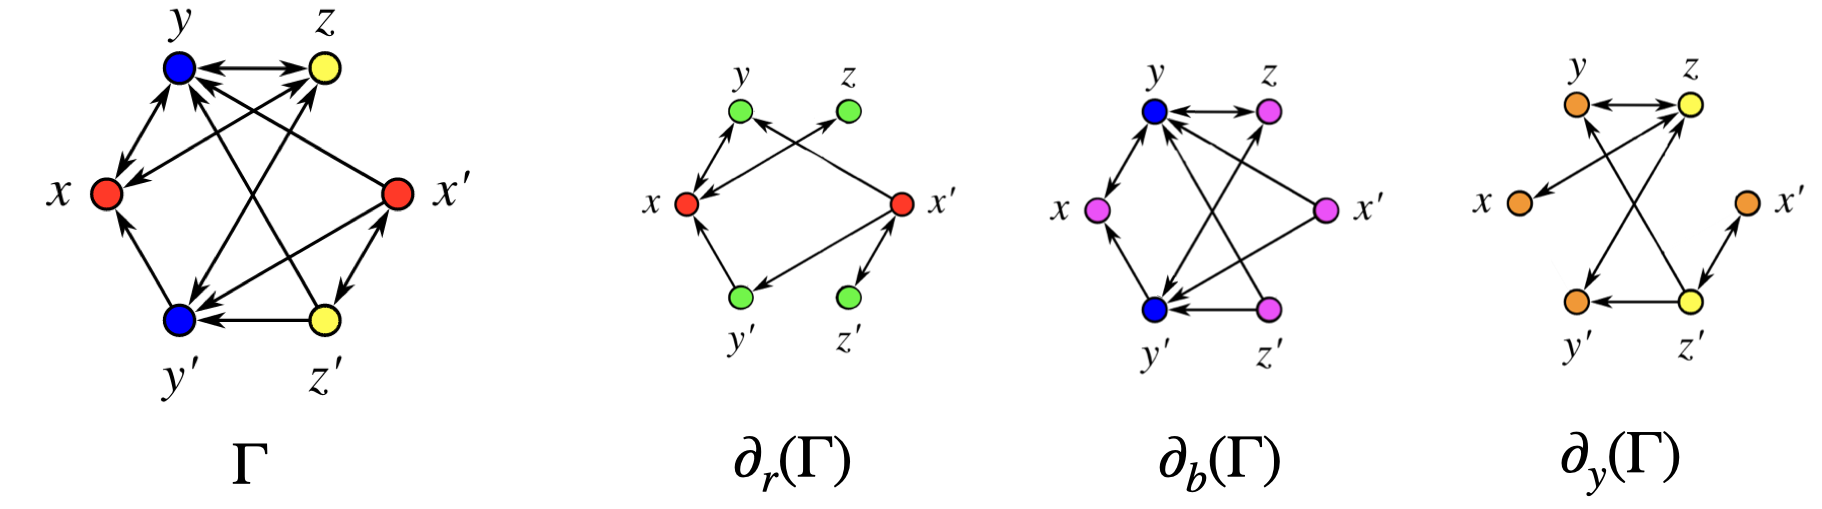
\includegraphics[width=16cm]{figures/color_derivatives.png}
    \caption{Color derivatives of a 3-BMG.}
      \label{fig:color_derivatives}
\end{figure}

Digraph $\Gamma$ in Figure~\ref{fig:color_derivatives} is a 3-BMG. However, none of its color derivatives are 2-BMGs, as they all contain either an induced F1-subgraph or an induced F2-subgraph. Indeed, $x'\rightarrow y'\rightarrow x$ and $z\rightarrow x$ define an induced F1-subgraph for $\partial_r(\Gamma)$; an induced F2-subgraph for $\partial_b(\Gamma)$ is given by $y'\rightarrow x\rightarrow y\rightarrow z\rightarrow y'$; the edges $x'\rightarrow z'\rightarrow y'$ and $z \rightarrow y'$ define an induced F1-subgraph for $\partial_y(\Gamma)$.
\end{example}

In case the color derivatives of a 3-colored digraph are 2-BMGs, they may not behave as excepted. For instance, the associated uncolored trees may not coincide, as it is shown in the following example. 

\begin{example}
\label{ex:2BMGcolor-derivative_no3BMG}
\begin{figure}[ht]
  \centering
    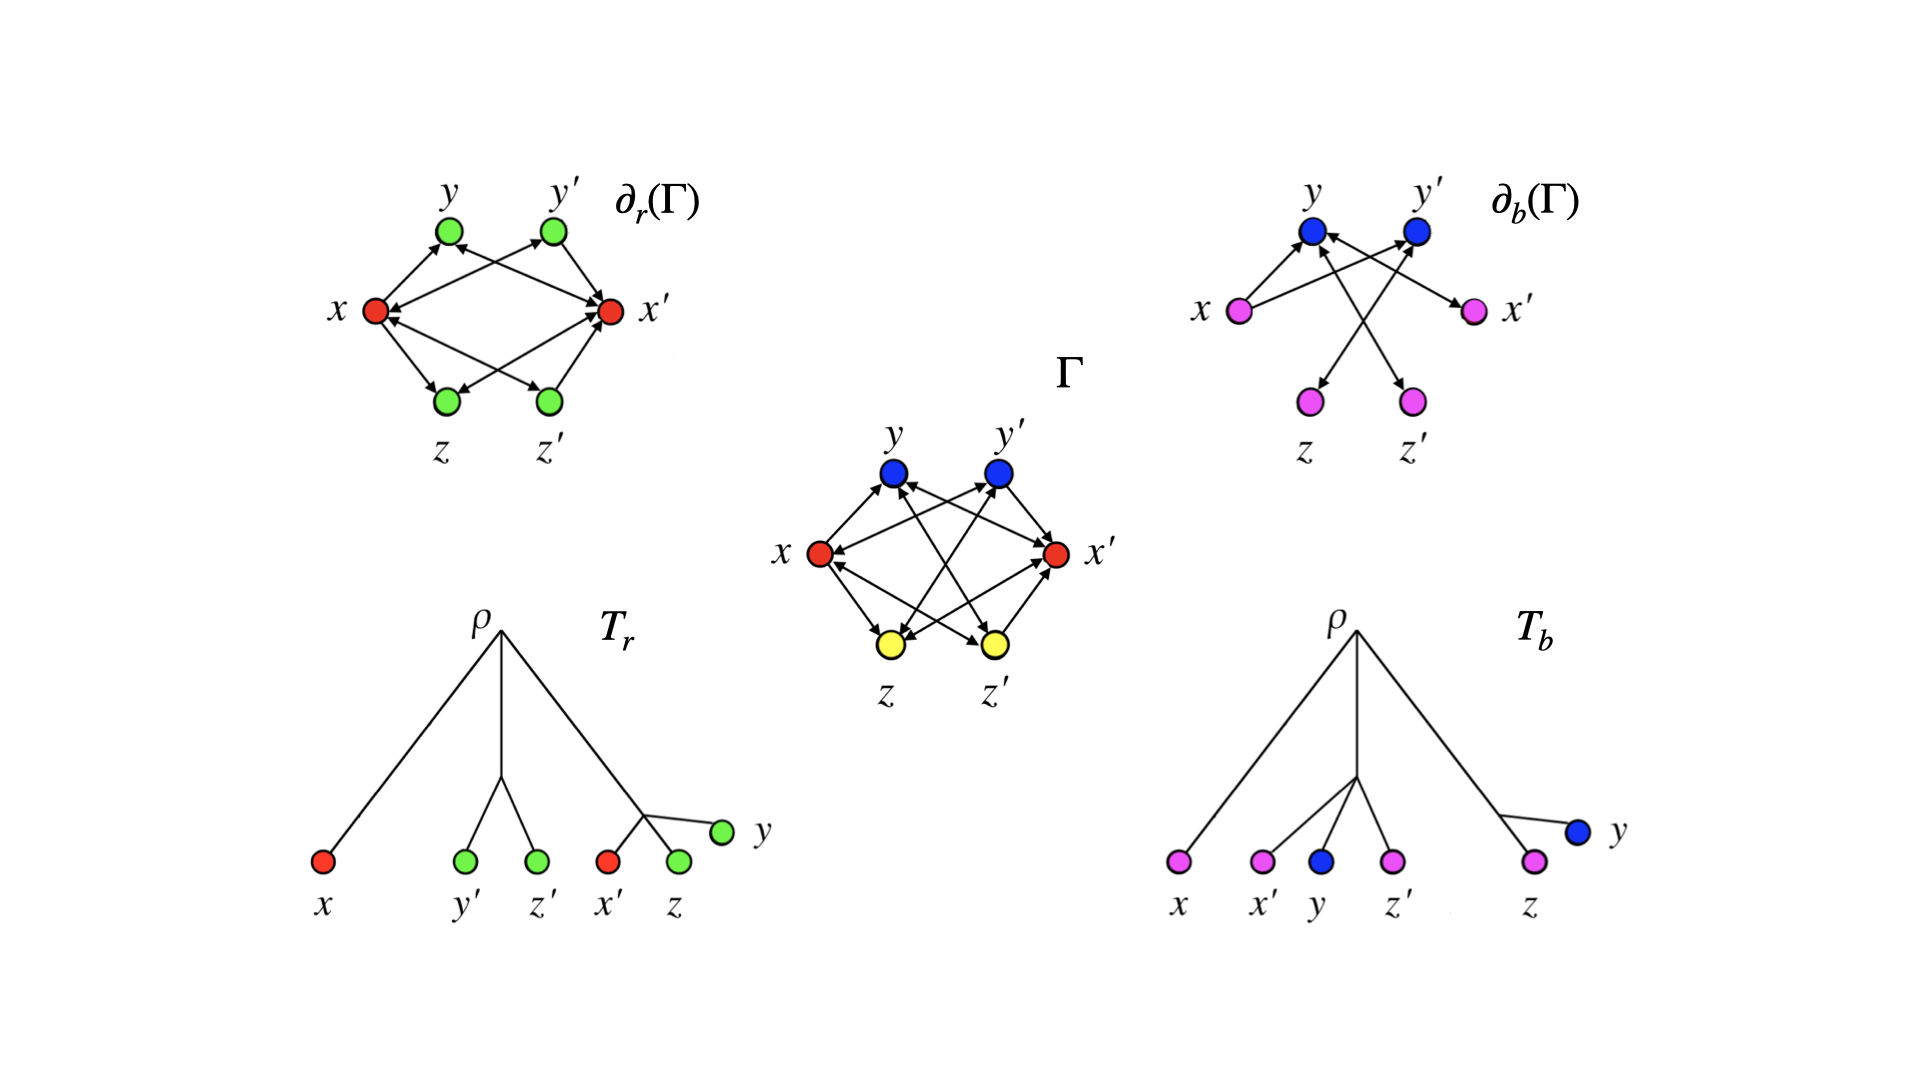
\includegraphics[width=16cm]{figures/different_trees.png}
    \caption{Red- and blue-derivative of $\Gamma$ which is not 3-BMG. The tree $T_r$ explains $\partial_r(\Gamma)$ while the tree $T_b$ explains $\partial_b(\Gamma)$.}
    \label{fig:different_trees}
\end{figure}

In Figure~\ref{fig:different_trees}, the uncolored trees associated to $T_r$ and $T_b$ are isomorphic but  do not coincide. Let $t$ be the parent of $y'$ in $T_r$, and let $t'$ be the parent of $y$ in $T_b$. The bijection $\phi:V(T_r)\rightarrow V(T_b)$ defined by $\phi(t)=t',\phi(z')=z$ and $\phi(v)=v$ for any $v\in V(T_r)$, is a tree isomorphism.  
Furthermore, $\Gamma$ is not a 3-BMG, as it contains an induced F2-subgraph, namely $x\rightarrow y$ together with $y\rightarrow x'\leftarrow y'$. 
\end{example}

Therefore, we introduce the \emph{color-delta operator} $\Delta_{rb}$ to characterize the case when $T_r$ and $T_b$ have the same uncolored tree.

\begin{definition}
\label{def:delta_operator}
Let $(\Gamma,\sigma)$ be a 3-colored digraph with colors red, blue, yellow, and color sets $R,B,Y$ respectively.
Let $(\Sigma,\sigma_r)$ be the 2-colored digraph on the vertex set of $\Gamma$ such that
\begin{equation}\label{def:sigma-r}
\sigma_r(v)= \begin{cases} 
      red & v\in R \\
     green & v\in B \,\dot{\cup}\, Y.
   \end{cases}
\end{equation}
Then
$(\Delta_{rb}(\Sigma),\sigma_b)$ is defined to be the 2-colored digraph on the vertex set of $\Gamma$ such that
\begin{equation}\label{def:sigma-b}
\sigma_b(v)= \begin{cases} 
    blue & v\in B \\
     pink & v\in R \,\dot{\cup}\, Y.
   \end{cases}
\end{equation}
 \end{definition}
We stress that $\partial_b(\Gamma)$ and $\Delta_{(r,b)}(\partial_r(\Gamma))$ have the same vertex set with the same coloring but they may have different edge sets. 

\begin{remark}
\label{obs:delta_operator}
$T_r$ and $T_b$ have the same uncolored tree if and only if $\Delta_{rb}(\partial_r(\Gamma))=\partial_b(\Gamma)$. In this case, the following diagram commutes.
\begin{figure}[ht]
  \centering
\begin{tikzcd}
(\partial_b(\Gamma),\sigma_b) 
& [3em](\Gamma,\sigma) \arrow{l}[sloped,above]{\text{}} \arrow[r]
& [3em](\partial_r(\Gamma),\sigma_r) \arrow[d,blue] \arrow[ll,{bend left=30},"\Delta_{(r,b)}",red]\\
[3em](T_r,\sigma_b)\arrow[u, blue] &[2em]  (T_r,\sigma)\arrow[l,blue] 
& [3em] (T_r,\sigma_r) \arrow[l,blue]
\end{tikzcd}
\caption{The red and blue arrows define the commutative diagram. Vertical maps between graphs and trees associate 2-BMGs and their explaining trees.}
\label{fig:diagram}
\end{figure}
\end{remark}

\subsection{3-BMG condition}
\label{sec:3-BMG condition}
In this section, we will show how color operators may be used to give a sufficient condition for a 3-colored digraph to be a 3-BMG.

\begin{theorem}\label{thm:sufficient_condition}
Let $(\Gamma,\sigma)$ be a 3-colored digraph with colors red, blue, yellow, and color sets $R,B,Y$ respectively. If $\partial_r(\Gamma)$ and $\partial_b(\Gamma)$ are 2-BMGs, and $\partial_b(\Gamma)=\Delta_{rb}(\partial_r(\Gamma))$, then $\Gamma$ is a 3-BMG.
\end{theorem}

\begin{proof}
We begin by showing that $\Gamma$ is color-sink free. If a vertex $x\in V$ is red then it has an out-neighbour in $\partial_{r}(\Gamma)$. Since $\partial_{r}(\Gamma)$ is a 2-BMG by hypothesis, this yields that $x$ is not a sink of $\partial_{r}(\Gamma)$ and hence neither of $\Gamma$. For a blue vertex $x$, the hypothesis that $\partial_b(\Gamma)$ is a 2-BMG yields that it is sink free, and hence some red or yellow vertex is an out-neighbor of $x$ in $\Gamma$. For a yellow vertex $x$, the last argument still applies showing that some red or blue vertex is an out-neighbor of $x$ in $\Gamma$. Thus, $\Gamma$ is sink free.

Since $\partial_{r}(\Gamma)$ is supposed to be a 2-BMG, $T_r$ is a tree explaining it, and its leaves are red or green colored as in Definition~\ref{def:delta_operator}. By~\cite[Proposition~2.3]{korchmaros2021quasi}, to prove that $\Gamma$ is a 3-BMG is enough to show that $(T_r,\sigma)$ displays all informative but none of the forbidden triples of $(\Gamma,\sigma)$, so that the pair $(\mathscr{R}(\Gamma),\mathscr{F}(\Gamma))$ is consistent.

Let $ab|b'$be a triple of $\Gamma$ such that $\sigma(a)\ne \sigma(b)=\sigma(b')$ and $ab\in E(\Gamma)$. We have to prove that $(T_r,\sigma)$ displays $ab|b'$ if $ab'\notin E(\Gamma)$ ($ abb'$ is informative) and does not display $ab|b'$otherwise ($ab|b'$is forbidden). Suppose that either $a$ or $b$ is a red vertex. Then $ab|b'\in \mathscr{R}(\partial_{r}(\Gamma))$ if $ab|b'$is informative, and $ab|b'\in \mathscr{F}(\partial_{r}(\Gamma))$ if $ab|b'$is forbidden, as $\partial_{r}$ preserves all edges headed or tailed on a red vertex and $\sigma_r(a)\ne \sigma_r(b)=\sigma_r(b')$. Hence, in the former case $ab|b'$ is displayed in $(T_r,\sigma_r)$ and the latter case $ab|b'$is not displayed in $(T_r,\sigma_r)$. This follows from~\cite[Proposition~2.3]{korchmaros2021quasi} since $\partial_{r}(\Gamma)$ is a 2-BMG. Assume neither $a$ nor $b$ is a red vertex; therefore, one between $a$ and $b$ is blue colored, and the previous argument shows that $ab|b'$ is displayed in $(T_b,\sigma_b)$ if $ab|b'$is informative, and $ab|b'$is not displayed in $(T_b,\sigma_b)$ if $ab|b'$is forbidden in $\Gamma$. Condition $\partial_b(\Gamma)=\Delta_{rb}(\partial_r(\Gamma))$ ensures that $T_r$ and $T_b$ have the same uncolored tree. Hence, $ab|b'$ is displayed in $(T_r,\sigma)$ if $ab|b'$is informative, and $ab|b'$is not displayed in $(T_r,\sigma)$ if $ab|b'$is forbidden.
\end{proof}

The 3-BMG condition only requires that two of the possible three color derivative graphs are 2-BMGs, assuming that they have the same uncolored explaining tree. This condition cannot be dropped as shown in Example~\ref{ex:2BMGcolor-derivative_no3BMG}. However, such a condition guaranties that also the yellow-color derivative of $\Gamma$ is a 3-BMG, as proven in the following proposition. 

\begin{proposition}\label{prop:yellow-derv}
Let $(\Gamma,\sigma)$ be a 3-colored digraph with colors red, blue, yellow, and color sets $R,B,Y$ respectively. If $\partial_r(\Gamma)$ and $\partial_b(\Gamma)$ are 2-BMGs, and $\partial_b(\Gamma)=\Delta_{rb}(\partial_r(\Gamma))$, then $\partial_{y}(\Gamma)$ is a 2-BMG.
\end{proposition}
\begin{proof}
Denote by $\sigma_y$ the color map that preserves the color of the vertices in $Y$, while it colors in orange all other vertices.
The arguments in the proof of Theorem~\ref{thm:sufficient_condition} yield $(\partial_{y}(\Gamma),\sigma_y)$ being sink-free. 

By~\cite[Proposition~2.3]{korchmaros2021quasi}, the yellow derivative $\partial_{y}(\Gamma)$ is a 2-BMG whenever $(T_r,\sigma_y)$ displays any informative triple of $\partial_{y}(\Gamma)$ and does not display any forbidden triple of $\partial_{y}(\Gamma)$. Let $ab|b'$be a triple of $\partial_{y}(\Gamma)$ such that $\sigma_y(a)\ne \sigma_y(b)=\sigma_y(b')$ and $ab\in E(\partial_{y}(\Gamma))$. Suppose that either $\sigma(a)$ or $\sigma(b)$ is a red, then $ab\in E(\partial_{r}(\Gamma))$ up to changing colors (from yellow and orange to red and green); hence, $ab|b'$is a triple of $\partial_{r}(\Gamma)$. Moreover $ab|b'$is informative (forbidden) in $\partial_{r}(\Gamma)$ if $ab|b'$is informative (forbidden) in $\partial_{y}(\Gamma)$, as the red-color derivative preserves all the neighbors in $\Gamma$ of a red vertex. Since $\partial_{r}(\Gamma)$ is supposed to be a 2-BMG, if $ab|b'$is informative in $\partial_{y}(\Gamma)$ then $ab|b'$ is displayed in $(T_r,\sigma_r)$ and then in $(T_r,\sigma_y)$. We also have that if $ab|b'$is forbidden in $\partial_{y}(\Gamma)$ then $ab|b'$is not displayed in $(T_r,\sigma_r)$ and then not in $(T_r,\sigma_y)$.

Assume that neither $\sigma(a)$ nor $\sigma(b)$ is a red, therefore one of them is of blue color in $\Gamma$, and then $ab\in E(\partial_{b}(\Gamma))$ up to changing colors (from yellow and orange to blue and pink); hence, $ab|b'$is a triple of $\partial_{b}(\Gamma)$. Using the previous argument, $(T_r,\sigma_y)$ displays any informative triple of $\partial_{y}(\Gamma)$ and does not display any forbidden triple of $\partial_{y}(\Gamma)$ where at least one of the vertices is of blue color.
\end{proof}

\section{Some necessary conditions for 3-BMGs}
\label{sec:nec_condition}
In general, the 3-BMG condition in Theorem~\ref{thm:sufficient_condition} is not necessary; indeed the color derivatives of a 3-BMG may not be 2-BMGs, as it is shown in Example~\ref{ex:color-derNo2BMG_3BMG}. 
Our interest in characterizations of 3-BMGs gives a motivation to search for a family of 3-BMGs with 2-BMG color derivatives.
In this section, we explore sufficient conditions in terms of color derivatives that lead to a large family of 3-BMGs characterized by the 3-BMG condition. 

\subsection{Color nuclei}
We begin by introducing the concept of \emph{color nucleus} of a 3-BMG. 
\begin{definition}
Let $(\Gamma,\sigma)$ be a 3-BMG with colors red, blue, yellow, and color sets $R,B,Y$ respectively, explained by $(T,\sigma)$. The $red_T${\emph{-nucleus}} $\Gamma_r$ of $\Gamma$ is the 2-BMG explained by $(T,\sigma_r)$ where $\sigma_r$ is defined as in (\ref{def:sigma-r}). The $blue_T$ and $yellow_T${\emph{-nucleus}} of $\Gamma$ are analogously defined and denoted by $\Gamma_b$ and $\Gamma_y$, respectively. 
\end{definition}
The term \emph{s-nucleus} denotes $\Gamma_s$ for any color $s$ of the vertices of $\Gamma$, and all s-nuclei of $\Gamma$ are also named \emph{color nuclei}. Figure~\ref{fig:color_nuclei} shows all color nuclei of the 3-BMG in Figure~\ref{fig:color_derivatives}.
\begin{figure}[ht]
  \centering
    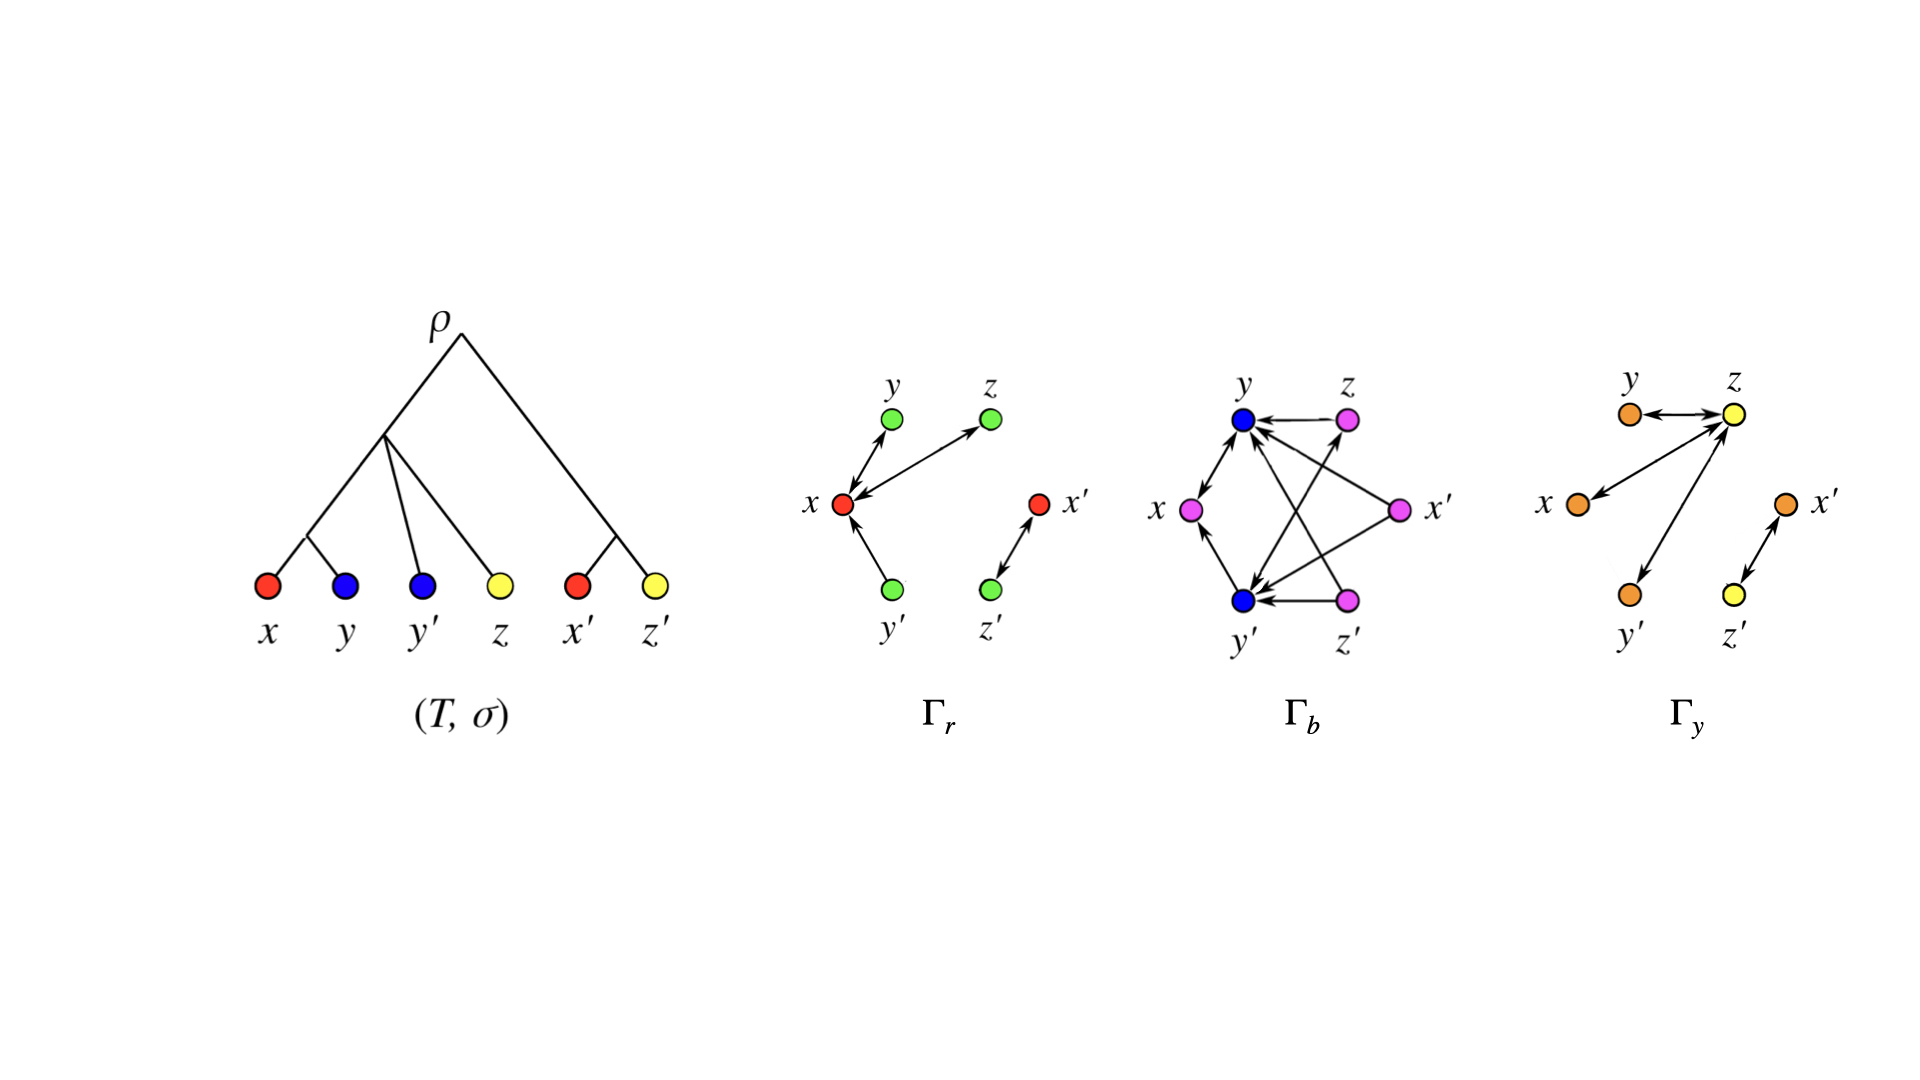
\includegraphics[width=16cm]{figures/color_nuclei.jpeg}
    \caption{Color nuclei of a 3-BMG explained by $(T,\sigma)$. The graph $\Gamma$ in Figure~\ref{fig:color_derivatives} is explained by $T$.}
      \label{fig:color_nuclei}
\end{figure}
The s-derivative of $(\Gamma,\sigma)$ preserves all neighbours of any vertex $x$ with $\sigma(x)=s$. This is not always the case for the s-nucleus, and all possible scenarios are described in the following lemma. 
\begin{lemma}
\label{lemma:neighbours_condition}
Let $(\Gamma,\sigma)$ be a 3-BMG with colors red, blue, yellow, and color sets $R,B,Y$ respectively. For every red vertex $x$, one of the following cases occurs.
\begin{itemize}
\item[(i)] $N_{\Gamma_r}(x)=N_{\Gamma}^{B}(x)$;
\item[(ii)] $N_{\Gamma_r}(x)=N_{\Gamma}^{Y}(x)$;
\item[(iii)] $N_{\Gamma_r}(x)=N_{\Gamma}^{B}(x)\cup N_{\Gamma}^{Y}(x)$;
\end{itemize}
\end{lemma}
\begin{proof} 
Assume $(\Gamma,\sigma)$ is explained by the tree $(T,\sigma)$. Now, take $y\in N_{\Gamma}^{B}(x)$ and $z\in N_{\Gamma}^{Y}(x)$, as $\Gamma$ is sink-free.  We have one the following three possibilities:
\begin{itemize}
\item[(I)] $\lca(x,y)\prec_T \lca(x,z)$;
\item[(II)] $\lca(x,z)\prec_T \lca(x,y)$;
\item[(III)] $\lca(x,y)=_T \lca(x,z)$.
\end{itemize}
To prove the statement, we use the fact that the out-neighbors of a vertex $x \in R$ in $\Gamma_r$ are also out-neighbors of $x$ in $\Gamma$ (the viceversa is not always true).
If (I) occurs $xz\not\in E(\Gamma_r)$, as $\sigma_r(y)=\sigma_r(z)$. Take any $z'$ from $N_{\Gamma}^{Y}(x)$. Then $\lca(x,z)=_T \lca(x,z')$ and hence (I) also holds for $z'$. Similarly, (II) implies $xy'\not\in E(\Gamma_r)$ for any $y'\in N_{\Gamma}^{B}(x)$. Moreover, in case of (III),  $xy\in E(\Gamma)$ if and only if $xz\in E(\Gamma)$ and hence $xy\in E(\Gamma_r)$ if and only if $xz\in E(\Gamma)$. The claim follows from  $\lca(x,y')=_T \lca(x,y)=_T\lca(x,z)=_T \lca(x,z')$ for any $y'\in N_{\Gamma}^{B}(x)$ and $z'\in N_{\Gamma}^{Y}(x)$.
\end{proof}

It may be noted that if $\Gamma$ is the 3-BMG in Figure~\ref{fig:color_derivatives}, then each of its color nuclei is strictly contained in its corresponding color derivative. Actually, this is true in general, and the two graphs coincide when the color derivative is a 2-BMG.

\begin{proposition}
\label{prop:nucleus2BMG}
Let $(\Gamma,\sigma)$ be a 3-BMG with colors red, blue, yellow, and color sets $R,B,Y$ respectively, explained by $(T,\sigma)$. Then $\Gamma_r\subseteq \partial_r(\Gamma)$, and $\Gamma_r$ coincides with $\partial_r(\Gamma)$ if the red derivative is a 2-BMG.
\end{proposition}
\begin{proof}
First, observe that red-nucleus and derivative have the same vertex set $V=L(T)$ and vertex coloring $\sigma_r$. Merging vertices in $\Gamma$ and leaves in $T$ always preserves the red out-neighbours in $B\cup Y$. However, from Lemma~\ref{lemma:neighbours_condition}, red vertices may lose some blue or yellow out-neighbours in $\Gamma_r$. Hence, $\Gamma_r$ is an induced subgraph of $\partial_r(\Gamma)$.

Suppose $\partial_r(\Gamma)$ is a 2-BMG. By definition of red-nucleus, $(T,\sigma_r)$ explains $\Gamma_r$. Suppose that $(T_r,\sigma^*)$ explains the red derivative of $\Gamma$.
Since $L(T)$ and $L(T_r)$ coincide and $\sigma^*=\sigma_r$, the claim $T_r=T$ actually reads $(T_r,\sigma_r)=(T, \sigma^*)$. Therefore, it suffices to prove that all informative triples in $\mathscr{R}(\Gamma_r)$ are displayed in $T_r$ but none of the forbidden triples in $\mathscr{F}(\Gamma_r)$ are displayed in $T_r$.

Let $ab|b'\in \mathscr{R}(\Gamma_r)$. Then $ab\in E(\Gamma_r)$ but $ab'\not\in E(\Gamma_r)$. From Lemma~\ref{lemma:neighbours_condition}, $ab\in E(\Gamma_r)$ implies $ab\in E(\Gamma)$. Since $\sigma_r(a)=\sigma^*(a)$ and $\sigma_r(b)=\sigma_r(b')=\sigma^*(b')=\sigma^*(b)$, this yields
$ab\in E(\partial_r(\Gamma))$. Assume on the contrary $ab'\in E(\partial_r(\Gamma))$. Then $ab'\in E(\Gamma)$ together with $ab\in E(\Gamma_r)\subset E(\Gamma)$ yields that $ab|b'$is a forbidden triple in $(T,\sigma)$. But this a contradiction as $(T,\sigma_r)$ also explains $\Gamma_r$.
Let $ab|b'\in\mathscr{F}(\Gamma_r)$. Then $ab\in E(\Gamma_r)$ and $ab'\in E(\Gamma_r)$. Thus $ab\in E(\Gamma)$ and $ab'\in E(\Gamma)$ whence $ab\in E(\partial_r(\Gamma))$ and $ab'\in E(\partial_r\Gamma))$. Therefore $ab|b'$is a forbidden triple of $\partial_r(\Gamma)$.
\end{proof}

\begin{remark}
\label{rm:derivative2nucleus}
Lemma~\ref{lemma:neighbours_condition} together with Proposition~\ref{prop:nucleus2BMG} yields a procedure to obtain color nuclei from their corresponding color derivatives. Indeed, the arguments of Proposition~\ref{prop:nucleus2BMG} proves that the subgraph induced by $B \cup Y$ is common to the red-nucleus and red-derivative, and we only need to delete the out-neighbours of any red vertex according to the arguments of Lemma~\ref{lemma:neighbours_condition}. In case (I), we have to remove from $\partial_r(\Gamma)$ the edges $xy$ with $y\in Y$, and in case (II) those with $y\in B$. If case (III) occurs, then no edge $xy$ has to be removed. 
\end{remark}
Now, we show that under certain circumstances, case (III) of Lemma~\ref{lemma:neighbours_condition} can only occur. 
\begin{proposition}
\label{prop:ch-2-BMGs-caseiii}
Let $(\Gamma,\sigma)$ be a 3-BMG with colors red, blue, yellow, and color sets $R,B,Y$ respectively. Then its red-derivative is a 2-BMG if and only if $N_{\Gamma_r}(x)=N_{\Gamma}^{B}(x)\cup N_{\Gamma}^{Y}(x)$ for every vertex $x\in R$.
\end{proposition}
\begin{proof}
From Remark~\ref{rm:derivative2nucleus}, if Case (III) in Lemma~\ref{lemma:neighbours_condition} occurs for any red vertex $x\in V$ then $\partial_r(T)=\Gamma_r$, and the red-derivative is a 2-BMG by definition of red-nucleus.

On the other hand, if $\partial_{r}(\Gamma)$ is a 2-BMG, then $\partial_{r}(\Gamma)=\Gamma_{r}$, as they are both explained by $(T,\sigma_r)$ by the arguments of Proposition~\ref{prop:nucleus2BMG}. Therefore, $N_{\Gamma_{r}}(x)= N_{\partial_{r}(\Gamma)}(x)=N_{\Gamma}^{B}(x)\cup N_{\Gamma}^{Y}(x)$ for all $x\in R$, as the red derivative preserves all neighbours of any red vertex.
\end{proof}
We have observed that the viceversa of Theorem~\ref{thm:sufficient_condition} is not true in general, as being a 3-BMG does not imply that the color derivatives are 2-BMGs; however, the second hypothesis in Theorem~\ref{thm:sufficient_condition} is guaranteed when the color derivatives are 2-BMGs. 
\begin{proposition}\label{prop:3BMGs_(D)}
Let $\Gamma$ be a 3-colored digraph such that $\partial_r(\Gamma)$ and $\partial_b(\Gamma)$ are 2-BMGs. If $(\Gamma,\sigma)$ is a 3-BMG explained by $(T,\sigma)$, then $\partial_b(\Gamma)=\Delta_{rb}(\partial_r(\Gamma))$.
\end{proposition}
\begin{proof}
If the red- and blue-derivative are 2-BMGs, they coincide with their corresponding nuclei by Proposition~\ref{prop:nucleus2BMG}; hence, they are explained by $(T,\sigma_r)$ and $(T,\sigma_b)$, respectively, where $\sigma_b$ is defined as in (\ref{def:sigma-b}). Therefore, $(T_r,\sigma_r)=(T,\sigma_r)$ and $(T_r,\sigma_b)=(T,\sigma_b)$ making the diagram in Figure~\ref{fig:diagram} commutative. Hence, $\partial_b(\Gamma)=\Delta_{rb}(\partial_r(\Gamma))$ by Remark~\ref{obs:delta_operator}.
\end{proof}

In case of 2-colored sink-free digraphs, Schaller et al.~\cite{schaller2021complexity} proved that 2-BMGs are characterized by forbidden three families of four vertices digraphs. In particular, 2-BMGs do not admit any directed 4-cycle~\cite[Theorem~4.4]{schaller2021complexity}. Now, we show that the same result holds true under the hypotheses of 3-BMG condition.     
\begin{proposition}
Let $(\Gamma,\sigma)$ be a 3-colored digraph with colors red, blue, yellow, and color sets $R,B,Y$ respectively. If $\partial_r(\Gamma)$ and $\partial_b(\Gamma)$ are 2-BMGs, and $\partial_b(\Gamma)=\Delta_{rb}(\partial_r(\Gamma))$, then $\Gamma$ does not admit any directed $4$-cycle.
\end{proposition}
\begin{proof}
Let $x_1\rightarrow x_2\rightarrow x_3 \rightarrow x_4 \rightarrow x_1$ be a directed $4$-cycle in $\Gamma$. Observe that at least two vertices in the cycle must have the same color, and assume that this color is red; hence, either $x_1,x_3\in R$ or $x_2,x_4\in R$ , as $\Gamma$ is properly vertex-colored. Now consider the subgraph induced by $\{x_1,\ldots, x_4\}$; this is contained in $\partial_r(\Gamma)$, as the red derivative preserves every neighbour of any red vertex. However, this contradicts the fact that 2-BMGs do not admit any directed 4-cycle~\cite[Theorem~4.4]{schaller2021complexity}.

Recall that $\partial_y(\Gamma)$ is also 2-BMG by Proposition~\ref{prop:yellow-derv}. Therefore, the previous argument applies to any colored directed 4-cycle.
\end{proof}

\subsection{Forbidden 3-vertex subgraphs}
\label{sec:forbidden_graphs}
In this section, we will show how avoiding certain 3-vertex configurations characterizes 3-BMGs in terms of the 3-BMG condition. 

\begin{definition}
\label{def:color-triangular}
A 3-colored digraph $\Sigma$ on three distinct vertices $\{x,y,z\}$ of different colors, red,blue,yellow, is an \emph{F$^R$-graph on a red vertex} $x$ if $xy,xz\in E(\Sigma)$ and $y$ and $z$ are adjacent. $\Sigma$ is an \emph{F$^R$-graph} if it is an F$^R$-graph on all its red vertices. F$^B$-graph and F$^Y$-graph are analogously defined. 
\end{definition}

F$^R$-graphs on a red vertex $x$ are induced subgraphs of a 3-BMG when case (i) in Lemma~\ref{lemma:neighbours_condition} occurs for $x$, as proven in the following lemma.
\begin{lemma}
\label{lemma:caseI-red_triangular}
Let $(\Gamma,\sigma)$ be a 3-BMG with colors red, blue, yellow, and color sets $R,B,Y$ respectively.  If $x$ is a red vertex such that $N_{\Gamma_r}(x)=N^B(x)$, then $\Gamma$ contains an induced F$^R$-subgraph on $x$.
\end{lemma}
\begin{proof}
$\Gamma$ is color-sink-free by~\cite[Proposition~2.3]{korchmaros2021quasi}. Let $y\in N^B(x)$ and $z\in N^Y(x)$. Since $N_{\Gamma_r}(x)=N^B(x)$, Case (I) in the proof of Lemma~\ref{lemma:neighbours_condition} yields $\lca(x,y)\prec \lca(x,z)$. Take $z'\in N^Y(y)$, and assume that $\lca(z',y)\preceq \lca(x,y)$. Then $\lca(x,z')=\lca(x,y)$. On the other hand, $\lca(x,z)\preceq \lca(x,z')$, as $z$ is a best match of $x$ and $\sigma(z)=\sigma(z')$, contradicting $\lca(x,y) \prec \lca(x,z)$. Therefore, we must have $\lca(x,y)\prec \lca(z',y)$.

Now, we show that $z\in N^Y(y)$. Assume on the contrary $z\notin N^Y(y)$. Then $\lca(z',y)\prec \lca(z,y)$, as $z'$ is a best match of $y$. This together with $\lca(x,y)\prec \lca(z',y)$ yield $z'\in N^Y(x)$. Hence, $\lca(x,z')=\lca(x,z)$ by $z\in N^Y(x)$. Finally, $\lca(y,z')=\lca(y,z)$, as $\lca(x,y)\prec \lca(z',y)$ and $\lca(x,y)\prec \lca(z,y)$. Therefore, $z\in N^Y(y)$.
\end{proof}

Up to interchanging blue and yellow colors, the arguments in the proof of Lemma~\ref{lemma:caseI-red_triangular} may be used to prove the following corollary.

\begin{corollary}
\label{cor:caseII-red_triangular}
Let $(\Gamma,\sigma)$ be a 3-BMG with colors red, blue, yellow and color sets $R,B,Y$ respectively. If $x$ is a red vertex such that $N_{\Gamma_r}(x)=N^Y(x)$, then $\Gamma$ contains an induced F$^R$-subgraph on $x$.
\end{corollary}

Therefore, avoiding F$^R$-subgraphs ensures that case (iii) in Lemma~\ref{lemma:neighbours_condition} holds for any red vertex.

\begin{proposition}
\label{prop:caseiii-suf_cond}
Let $(\Gamma,\sigma)$ be a 3-BMG with colors red, blue, yellow  and color sets $R,B,Y$ respectively. If $\Gamma$ does not contain any induced F$^R$-subgraph, then $N_{\Gamma_r}(x)=N^B(x)\cup N^Y(x)$ for every $x\in R$.
\end{proposition}
\begin{proof}
For any red vertex $x\in V(\Gamma)$, case (i) in Lemma~\ref{lemma:neighbours_condition} does not occur by Lemma~\ref{lemma:caseI-red_triangular}. Also, case (ii) in Lemma~\ref{lemma:neighbours_condition} does not occur by Corollary~\ref{cor:caseII-red_triangular}. Hence, $x$ must satisfy case (iii) in Lemma~\ref{lemma:neighbours_condition}, and $N_{\Gamma_r}(x)=N^B(x)\cup N^Y(x)$. 
\end{proof}

Proposition~\ref{prop:ch-2-BMGs-caseiii} together with Proposition~\ref{prop:caseiii-suf_cond} gives the following corollary.

\begin{corollary}
\label{cor:2BMGsD-forbidden}
Let $(\Gamma,\sigma)$ be a 3-BMG with colors red, blue, yellow, and color sets $R,B,Y$ respectively. If $\Gamma$ does not contain an induced F$^R$-subgraph, then $\partial_r(\Gamma)$ is a 2-BMG.
\end{corollary}

Theorem~\ref{thm:sufficient_condition} together with Proposition~\ref{prop:3BMGs_(D)} and Corollary~\ref{cor:2BMGsD-forbidden} gives a 3-BMG characterization for any 3-colored digraph free from induced F$^B$- and F$^R$-subgraphs.

\begin{theorem}\label{thm:characterization3BMG_forbidden}
Let $\Gamma$ be a 3-colored graph free from induced F$^B$- and F$^R$-subgraphs. Then $\Gamma$ is a 3-BMG if and only if $\partial_{r}(\Gamma)$ and $\partial_{b}(\Gamma)$ are 2-BMGs and $\partial_b(\Gamma)=\Delta_{rb}(\partial_r(\Gamma))$.
\end{theorem}

Theorem~\ref{thm:characterization3BMG_forbidden} begs the question whether a 3-BMG is free from induced F$^R$-subgraphs. This is not true in general. Indeed, the 3-BMG in Figure~\ref{fig:color_derivatives} has a F$^R$-subgraph, namely, $x \rightarrow y \rightarrow z$ together with $x\rightarrow z$.

\subsection{Symmetric edges}\label{sec:sym_edges}
In case $\Gamma$ has a symmetric edge incident a yellow vertex and a blue vertex, forbidding F$^R$-subgraphs may be rephrased in the following way.

\begin{remark}\label{rmk:sym_F^R}
Suppose that a 3-colored graph $\Gamma$ with colors red, blue, yellow vertices is free of F$^R$-subgraphs. Observe that if it has a symmetric edge incident a yellow and a blue vertex, then they cannot have a common in-neighbour. 
\end{remark}

Therefore, forbidding F$^R$-subgraphs restricts the possible common red in-neighbours of the vertices of a symmetric edge by Remark~\ref{rmk:sym_F^R}. In this section, we show that there is a symmetric edge for every pair of different colors in a BMG. Let us recall that BMGs are color-sink-free by~\cite[Proposition~2.3]{korchmaros2021quasi}. First, we will see when such a hypothesis ensures the presence of at least one symmetric edge. 

\begin{proposition}
\label{prop:sink-free_sym}
Let $\Gamma$ be a properly colored digraph which is color-sink-free. If $\Gamma$ has no directed cycle of length at least $3$, then $\Gamma$ has a symmetric edge.
\end{proposition}
\begin{proof} 
Let $x_1\rightarrow x_2\cdots\rightarrow x_{n-1}\rightarrow x_n$ be a directed path in $\Gamma$. Since $\Gamma$ is sink-free, $x_n$ has at least one out-neighbour, say $x_{n+1}\in V(\Gamma)$. If $x_{n+1}\neq x_i$ for all vertices in the path, add $x_{n+1}$ at the end of the path. Repeating this process gives an infinite sequence of vertices of $V(\Gamma)$, contradicting the finiteness of the vertex-set of $\Gamma$. Therefore, we may assume that $x_j=x_i$ for some $1\leq i<j$. Not having any directed cycle of length $\ge 3$ yields $j=i+1$, and then $x_i x_{i+1}$ is a symmetric edge of $\Gamma$.
\end{proof}

The lower bound on the length of the forbidden direct cycles in Proposition~\ref{prop:sink-free_sym} can be dropped when $\Gamma$ is a 2-BMG.

\begin{lemma}
\label{lemma:2BMG-sym}
Every directed cycle in a 2-BMG is a symmetric edge.
\end{lemma}
\begin{proof}
Let $\Gamma$ be a 2-colored bi-transitive digraph, and let $x_1\rightarrow x_2\rightarrow \cdots \rightarrow x_{n} \rightarrow x_1$ be a directed cycle of length $n>2$ in $\Gamma$. We prove that there is not such a cycle by induction on $n$; therefore, we must have $n=2$, and $x_1x_2$ is symmetric in $\Gamma$.

Since $\Gamma$ is a properly 2-colored digraph, it has no cycle of odd size; hence, $n\neq3,5$. Actually we have $n\neq4$, as directed $4$-cycles are prohibited in 2-BMGs by~\cite[Corollary~3.6]{schaller2021complexity}; hence, $n\geq 6$.

Now, assume that $\Gamma$ does not contain any directed $m$-cycle with $6\leq m<n$. Recall that 2-BMGs are bi-transitive; hence, $x_1x_4\in E(\Gamma)$. Therefore, there is also a directed $(n-2)$-cycle, namely, $x_1\rightarrow x_4\rightarrow \cdots \rightarrow x_{n} \rightarrow x_1$ in $\Gamma$, contradicting our inductive hypothesis.
\end{proof}

Actually, the following proposition shows that a 2-BMG always contain a symmetric edge. In the general case, there are at least as many symmetric edges as the number of pair of different colors  
\begin{proposition}
An n-BMG contains at least $\binom{n}{2}$ symmetric edges.
\end{proposition}
\begin{proof}
Suppose on the contrary that there are two colors, namely red and blue, such there is no symmetric edge connecting a red vertex to a blue vertex of $\Gamma$.

Let $x$ be a red vertex of $\Gamma$. There is a vertex $y$ in the blue out-neighbour of $x$, as $\Gamma$ is color-sink-free from~\cite[Proposition~2.3]{korchmaros2021quasi}. Since $xy$ is not symmetric, $y$ admits a red out-neighbour $x_1$ such that $x\neq x_1$. Now, choose a blue out-neighbour $y_1$ of $x_1$. Then, there is a red out-neighbour $x_2$ of $y_1$ such that $x_2\neq x_1$, as $x_1y_1$ is not symmetric. Repeating this construction leads to an infinite sequence of distinct vertices $\{x,x_1,x_2,\ldots\,x_n\}$, contradicting $|V(\Gamma)|< \infty$. Therefore, there are $i,j$ such that $1\leq i<j\leq n$ and $x_i=x_j$. We may assume $j-i>1$, otherwise we have a symmetric edge $x_iy_i$ with $y_i\in B$, contradicting the hypothesis. Hence, there is a directed 2-colored cycle in $\Gamma$, namely, $xyx_1y_1\cdots x_iy_i\cdots y_{j-1}x_i$. From~\cite[Theorem~9]{schaller2021corrigendum}, the subgraph of $\Gamma$ induced by the vertices of this cycle is a 2-BMG, contradicting Lemma~\ref{lemma:2BMG-sym}. Hence, there is at least one symmetric edge between a blue and red vertex of $\Gamma$.

The statement follows by observing that there are $\binom{n}{2}$ possible pairs of different colors among $n$ colors. 
\end{proof}

\label{sec:cycles}
\section{Summary and open problems}
In this contribution, we have seen how the idea of merging colors gives rise to a condition, called 3-BMG condition, which is sufficient for a 3-colored graph to be a 3-BMG. The 3-BMG condition means that (at least) two color derivatives of the 3-colored graph are 2-BMGs explained by the same uncolored tree. Example~\ref{ex:2BMGcolor-derivative_no3BMG} shows that 2-BMG color derivatives may not be explained by the same uncolored (labelled) tree but their uncolored trees are isomorphic. Every 2-BMG is uniquely explained by its least resolved tree (LRT)~\cite[Theorem 8]{Geiss:19a}. It remains open the question whether the uncolored LRTs of 2-BMG color derivatives are isomorphic.

In the opposite direction, to ensure that the red color derivative of a 3-BMG is a 2-BMG, it is required that the last common ancestor between every red vertex and its best match be color independent. This requirement is fulfilled when certain 3-colored digraphs on three vertices (so-called F$^R$-graphs) are forbidden in the 3-BMG.

For n-colored digraphs with $n>3$, the 3-BMG condition is naturally generalized to the n-BMG condition requiring that (at least) $n-1$ color derivatives are 2-BMGs explained by the same uncolored tree. As for $n=3$, the n-BMG condition is sufficient for n-colored digraphs to be n-BMGs. Whether it is still sufficient in a weaker form requiring the condition for less than $n-1$ colors is left as an open problem.

Symmetric edges play a key role when BMGs are used for detecting orthology genes~\cite{stadler2020pairs}. For any two colors, we have shown that there is a symmetric edge connecting two vertices of those colors. This motivates a graph-theoretic investigation of the BMGs with many symmetric edges. In this direction, ~\cite{geiss2020reciprocal} contains some results for the case where $n=3$ and all edges are symmetric. A related open problem is to give a characterization of 3-colored digraphs with the property that each vertex is incident to at least one symmetric edge. 


\bibliographystyle{elsarticle-num}
\bibliography{references}

\end{document}















